% !TeX program = xelatex
% Compile with XeLaTeX or LuaLaTeX to preserve Vietnamese Unicode text.
\documentclass[conference]{IEEEtran}
\IEEEoverridecommandlockouts
% The preceding line is only needed to identify funding in the first footnote. If that is unneeded, please comment it out.
%Template version as of 6/27/2024

\usepackage{fontspec}
\usepackage[english,vietnamese]{babel}
\defaultfontfeatures{Ligatures=TeX}


\usepackage{cite}
\usepackage{amsmath,amssymb,amsfonts}
\usepackage{algorithmic}
\usepackage{booktabs}
\usepackage{graphicx}
\usepackage{capt-of}
\usepackage{textcomp}
\usepackage{xcolor}
\usepackage[hidelinks]{hyperref}
\def\BibTeX{{\rm B\kern-.05em{\sc i\kern-.025em b}\kern-.08em
    T\kern-.1667em\lower.7ex\hbox{E}\kern-.125emX}}
\begin{document}
\selectlanguage{vietnamese}

\title{Khai thác tập mục phổ biến từ ảnh Fashion MNIST}

\author{\IEEEauthorblockN{Nhóm thực hiện Ứng dụng 2}}

\maketitle

\begin{abstract}
Báo cáo chuyển 70.000 ảnh Fashion-MNIST thành giao dịch túi từ thị giác nhị phân và khai thác tập mục phổ biến bằng hai backend Eclat. K-means với 32 cụm hội tụ sau 220 vòng; hai backend khớp kết quả ở cả sáu ngưỡng, với 6.185 tập mục tại ngưỡng hỗ trợ 5\%. Trong số này, 4.180 tập có hệ số làm giàu cao nhất theo lớp từ 2 trở lên. Đo một lượt ghi nhận BitVector nhanh hơn Set 2,40 lần ở ngưỡng 5\%, nhưng chưa đủ để kết luận về hiệu năng tổng quát. Do cả ảnh huấn luyện và kiểm thử được dùng để học từ điển và khai thác, kết quả chỉ hỗ trợ phân tích khai phá mẫu, không phải đánh giá phân loại độc lập.
\end{abstract}

\begin{IEEEkeywords}
Fashion-MNIST, túi từ thị giác nhị phân, Eclat, tập mục phổ biến.
\end{IEEEkeywords}

\section{Khai thác mẫu trực quan phổ biến trên Fashion-MNIST}

\subsection{Bài toán và tập dữ liệu}

Trong dữ liệu giao dịch, khai thác tập mục phổ biến giúp tìm những mục thường đi cùng nhau. Để áp dụng Eclat cho ảnh, nhóm biểu diễn mỗi vùng ảnh nhỏ bằng một từ thị giác (\textit{visual word}) và xem tập các từ xuất hiện trong một ảnh là một giao dịch. Mỗi tập mục phổ biến tìm được vì thế tương ứng với một tổ hợp từ thị giác thường cùng xuất hiện trong ảnh.

Tập dữ liệu \href{https://github.com/zalandoresearch/fashion-mnist}{Fashion-MNIST}~\cite{Xiao2017} gồm 70.000 ảnh xám kích thước $28 \times 28$ pixel, chia đều cho 10 lớp sản phẩm thời trang. Bảng~\ref{tab:fashionmnist_distribution} cho biết số ảnh của từng lớp trong hai tập gốc. Nhóm dùng cả hai tập để khai thác mẫu, đối chiếu một số mẫu với ảnh gốc và khảo sát mức độ phổ biến của chúng trong từng lớp.

Các ảnh có cùng kích thước nên có thể chia theo một lưới chung và đối chiếu các vùng được gán mã với ảnh gốc. Mỗi lớp có cùng số ảnh, giúp việc so sánh tỷ lệ xuất hiện của mẫu giữa các lớp dễ diễn giải.

\begin{table}[!t]
    \centering
    \caption{Số ảnh theo lớp trong Fashion-MNIST}
    \label{tab:fashionmnist_distribution}
    \footnotesize
    \setlength{\tabcolsep}{3pt}
    \begin{tabular}{@{}c l r r r@{}}
        \hline
        \textbf{Mã} & \textbf{Lớp} & \textbf{Huấn luyện} &
        \textbf{Kiểm thử} & \textbf{Tổng} \\
        \hline
        0 & T-shirt/top  & 6.000 & 1.000 & 7.000 \\
        1 & Trouser      & 6.000 & 1.000 & 7.000 \\
        2 & Pullover     & 6.000 & 1.000 & 7.000 \\
        3 & Dress        & 6.000 & 1.000 & 7.000 \\
        4 & Coat         & 6.000 & 1.000 & 7.000 \\
        5 & Sandal       & 6.000 & 1.000 & 7.000 \\
        6 & Shirt        & 6.000 & 1.000 & 7.000 \\
        7 & Sneaker      & 6.000 & 1.000 & 7.000 \\
        8 & Bag          & 6.000 & 1.000 & 7.000 \\
        9 & Ankle boot   & 6.000 & 1.000 & 7.000 \\
        \hline
          & \textbf{Tổng} & \textbf{60.000} & \textbf{10.000} & \textbf{70.000} \\
        \hline
    \end{tabular}
\end{table}

\subsection{Xây dựng cơ sở dữ liệu giao dịch từ ảnh}

Hình~\ref{fig:fashion_tc_pipeline} tóm tắt các bước chuyển ảnh Fashion-MNIST thành cơ sở dữ liệu giao dịch bằng BoVW nhị phân.

\begin{figure*}[!t]
    \centering
    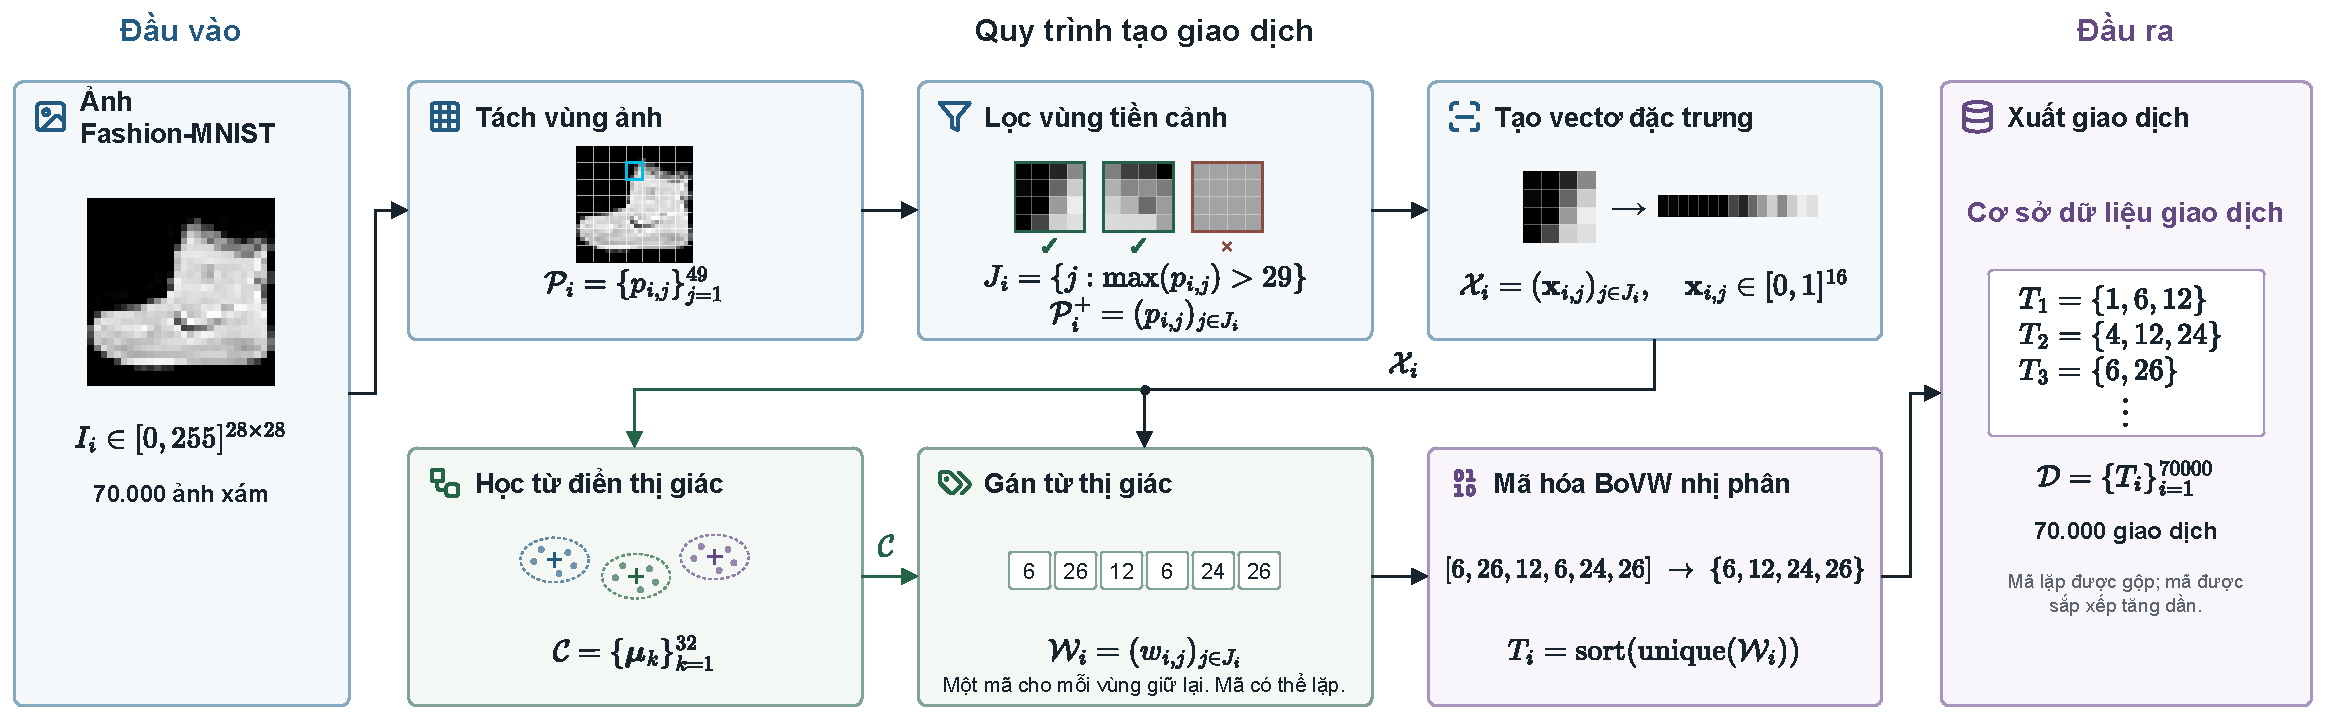
\includegraphics[width=\textwidth]{figures/diagram/TC_pipeline.pdf}
    \caption{Quy trình tạo giao dịch từ ảnh Fashion-MNIST. Nhóm học một từ điển chung từ các vùng giữ lại trên toàn bộ 70.000 ảnh rồi dùng từ điển đó để gán mã cho từng vùng. Các mã và giao dịch trong hình dùng để minh họa.}
    \label{fig:fashion_tc_pipeline}
\end{figure*}

Nhóm tạo giao dịch theo phương pháp túi từ thị giác (\textit{Bag of Visual Words}, BoVW)~\cite{Sivic03}. Mỗi ảnh được chia thành 49 vùng $4 \times 4$ pixel không chồng lấn. Trong bước khám phá dữ liệu, khi cả hai lưới đều loại khoảng 39,3\% số vùng, lưới $4\times4$ chỉ mất 5,92\% tổng độ lớn gradient, so với 14,00\% ở lưới $7\times7$. Kết quả này là cơ sở để chọn lưới $4\times4$ cho bước lọc nền.

Để lọc nền, nhóm chọn ngưỡng 29, tức phân vị 10\% của các điểm ảnh có giá trị lớn hơn 0 (Q10+). Quy tắc giữ vùng có ít nhất một điểm ảnh vượt ngưỡng loại 37,50\% số vùng và làm mất 4,41\% tổng độ lớn gradient. Mọi ảnh đều còn vùng sau khi lọc, với tổng cộng 2.143.746 trên 3.430.000 vùng được giữ. Trong mỗi vùng giữ lại, nhóm đọc 16 giá trị mức xám theo thứ tự cột rồi chia cho 255 để tạo vectơ trong $[0,1]^{16}$.

Nhóm dùng K-means~\cite{Hartigan1979} để phân cụm toàn bộ các vectơ thu được. Mỗi tâm trong 32 cụm là một từ trong từ điển thị giác. Sau khi học từ điển, nhóm gán cho mỗi vùng ảnh mã của tâm cụm gần nhất theo bình phương khoảng cách Euclid. Bảng~\ref{tab:kmeans_configuration} tóm tắt cấu hình K-means.

\begin{table}[!t]
    \centering
    \caption{Cấu hình K-means để xây dựng từ điển thị giác}
    \label{tab:kmeans_configuration}
    \footnotesize
    \setlength{\tabcolsep}{3pt}
    \begin{tabular}{@{}p{0.39\columnwidth} p{0.56\columnwidth}@{}}
        \hline
        \textbf{Tham số} & \textbf{Giá trị} \\
        \hline
        Phương pháp & K-means toàn bộ, khởi tạo K-means++ \\
        Dữ liệu phân cụm & Các vùng được giữ lại từ 70.000 ảnh \\
        Vectơ đặc trưng & 16 giá trị pixel xám đã chuẩn hóa \\
        Số cụm ($K$) & 32 \\
        Giá trị khởi tạo bộ sinh số ngẫu nhiên & 123 \\
        Độ đo khoảng cách & Bình phương khoảng cách Euclid \\
        Giới hạn lặp / dung sai & 300 / $10^{-4}$ \\
        Kết quả phân cụm & Hội tụ sau 139 vòng, cả 32 cụm đều có dữ liệu \\
        Quy tắc gán từ thị giác & Chọn tâm cụm gần nhất \\
        \hline
    \end{tabular}
\end{table}

Nhóm khảo sát $K=16,32,64,128,256$. Độ méo là trung bình của bình phương khoảng cách từ mỗi vectơ đến tâm cụm gần nhất. Với cùng giá trị khởi tạo ngẫu nhiên 123, độ méo ở $K=16,32,64$ lần lượt là 0,441, 0,347 và 0,271. Số mã trung bình mỗi giao dịch tăng tương ứng từ 9,00 lên 12,27 và 15,11. Nhóm chọn $K=32$ để giảm độ méo so với $K=16$ và giữ giao dịch ngắn hơn $K=64$.

Ở bước cuối, nhóm dùng BoVW nhị phân để tạo giao dịch $T_i$ cho ảnh $I_i$. Giao dịch chỉ ghi sự hiện diện của từng mã, theo thứ tự tăng dần. Tọa độ vùng ảnh được lưu riêng để đối chiếu khi diễn giải mẫu. Bộ dữ liệu có 70.000 giao dịch, mỗi giao dịch chứa từ 2 đến 26 mã, với trung vị 12 và trung bình 12,27. Phụ lục~\ref{app:fashion_configuration} trình bày khảo sát cấu hình và thống kê bổ sung.

\subsection{Thiết kế thực nghiệm khai thác}

Eclat tổ chức dữ liệu theo chiều dọc~\cite{Zaki2000}. Với mỗi mã thị giác, thuật toán lưu danh sách số thứ tự các giao dịch có chứa mã đó. Với tập mã $X$, thuật toán lấy phần giao giữa các danh sách tương ứng; số giao dịch còn lại là số ảnh chứa đồng thời mọi mã trong $X$. Nhóm so sánh hai cách lưu các danh sách này trên cùng bộ giao dịch BoVW nhị phân: Set lưu các số thứ tự hiện diện, còn BitVector biểu diễn chúng bằng các bit và lấy phần giao bằng phép AND.

Thực nghiệm dùng sáu ngưỡng hỗ trợ tối thiểu (\textit{minsup}), từ 80\% đến 5\%. Bảng~\ref{tab:fim_minsup} quy đổi mỗi ngưỡng thành số giao dịch cần có trên tổng số 70.000 giao dịch.

\begin{table}[!t]
    \centering
    \caption{Các ngưỡng hỗ trợ tối thiểu dùng trong thực nghiệm}
    \label{tab:fim_minsup}
    \begin{tabular}{c r}
        \hline
        \textbf{Ngưỡng (\%)} & \textbf{Số giao dịch tối thiểu} \\
        \hline
        80 & 56.000 \\
        60 & 42.000 \\
        40 & 28.000 \\
        20 & 14.000 \\
        10 &  7.000 \\
         5 &  3.500 \\
        \hline
    \end{tabular}
\end{table}

Nhóm khảo sát sáu ngưỡng để theo dõi số lượng, độ dài của các tập mục và chi phí khai thác. Ngưỡng 80\% xét các mẫu có mặt trong phần lớn ảnh. Ngưỡng 5\% mở rộng phạm vi phân tích theo lớp và vẫn yêu cầu mỗi mẫu xuất hiện trong ít nhất 3.500 ảnh.

Ở mỗi ngưỡng, nhóm kiểm tra hai cách biểu diễn có trả về cùng các tập mục và cùng số giao dịch hỗ trợ cho từng tập hay không. Sau đó, nhóm so sánh thời gian chạy và bộ nhớ cực đại, đồng thời khảo sát số lượng và độ dài của các tập mục khi giảm ngưỡng.

\subsection{Kết quả khai thác tập mục phổ biến}
\label{subsec:fashion_fim_results}

Set và BitVector trả về cùng danh sách tập mục và cùng số giao dịch hỗ trợ ở cả sáu ngưỡng. Khi tính lại độ hỗ trợ của từng tập mục trả về bằng cách giao các mặt nạ giao dịch, mọi giá trị đều khớp với kết quả Eclat.

Bảng~\ref{tab:eclat_backend_comparison} ghi số tập mục, độ dài lớn nhất và thời gian của hai bản cài đặt. Tỷ số thời gian bằng thời gian của Set chia cho thời gian của BitVector. Giá trị lớn hơn 1 cho biết bản BitVector chạy nhanh hơn trong lượt đo.

\begin{table}[!t]
    \centering
    \caption{Kết quả khai thác và thời gian thực thi của Set và BitVector}
    \label{tab:eclat_backend_comparison}
    \scriptsize
    \setlength{\tabcolsep}{3pt}
    \begin{tabular}{c r c r r c}
        \hline
        \textbf{Ngưỡng} &
        \textbf{Số tập mục} &
        \shortstack{\textbf{Độ dài}\\\textbf{lớn nhất}} &
        \textbf{Set (s)} &
        \textbf{BitVector (s)} &
        \textbf{Tỷ số} \\
        \hline
        80\% &     0 & 0 &  6,13 & 8,18 & $0{,}75\times$ \\
        60\% &     2 & 1 &  6,10 & 7,15 & $0{,}85\times$ \\
        40\% &    15 & 2 &  6,08 & 6,08 & $1{,}00\times$ \\
        20\% &   174 & 3 &  6,12 & 6,10 & $1{,}00\times$ \\
        10\% & 1.275 & 5 &  9,14 & 8,14 & $1{,}12\times$ \\
         5\% & 7.228 & 6 & 13,17 & 8,20 & $1{,}61\times$ \\
        \hline
    \end{tabular}
\end{table}

Hình~\ref{fig:eclat_itemset_counts} cho thấy số tập mục tăng nhanh khi hạ ngưỡng. Ở 80\%, không có tập mục nào đạt ngưỡng. Ở 60\%, chỉ có hai tập đơn mục $\{6\}$ và $\{26\}$. Từ 40\% xuống 5\%, số tập mục tăng từ 15 lên 7.228. Khi hạ ngưỡng, các tập mục đã đạt ngưỡng cũ vẫn được giữ và những tập có độ hỗ trợ thấp hơn bắt đầu xuất hiện.

\begin{figure}[!t]
    \centering
    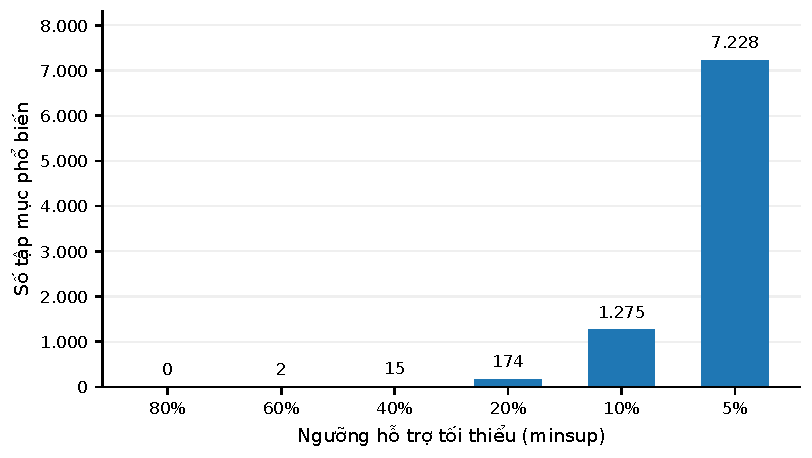
\includegraphics[width=\columnwidth]{figures/eclat/fig1_itemset_counts.pdf}
    \caption{Số tập mục phổ biến theo ngưỡng hỗ trợ tối thiểu.}
    \label{fig:eclat_itemset_counts}
\end{figure}

Ở ngưỡng 60\%, tập dài nhất chỉ có một mục. Đến ngưỡng 5\%, độ dài lớn nhất tăng lên sáu mục. Tuy vậy, phần lớn kết quả ở ngưỡng này là các tập ba hoặc bốn mục. Hai nhóm lần lượt có 2.481 và 3.178 tập, chiếm tổng cộng 78,29\% (Hình~\ref{fig:eclat_length_distribution}).

\begin{figure}[!t]
    \centering
    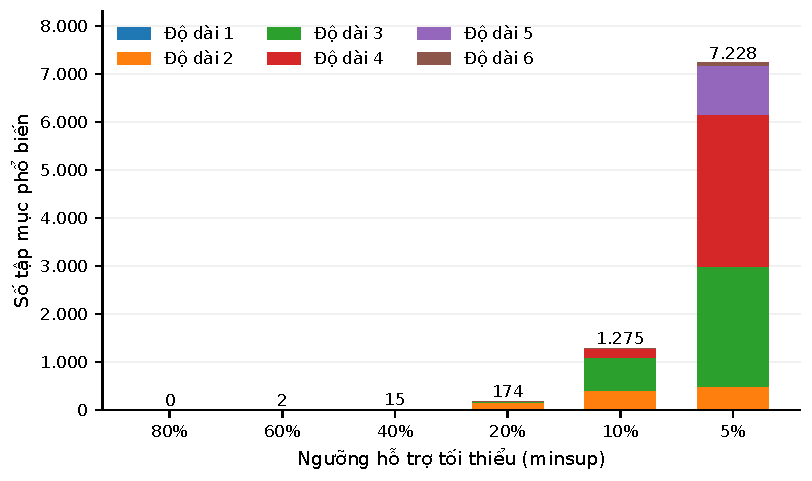
\includegraphics[width=\columnwidth]{figures/eclat/fig4_length_distribution.pdf}
    \caption{Phân bố độ dài tập mục theo ngưỡng hỗ trợ tối thiểu.}
    \label{fig:eclat_length_distribution}
\end{figure}

Set chạy nhanh hơn ở ngưỡng 80\% và 60\%, hai bản có thời gian gần bằng nhau ở 40\% và 20\%, còn BitVector chạy nhanh hơn ở 10\% và 5\% (Hình~\ref{fig:eclat_runtime}). Trong lượt đo ở 5\%, bản BitVector giảm 37,8\% tổng thời gian và 18,0\% bộ nhớ cực đại so với bản Set.

\begin{figure}[!t]
    \centering
    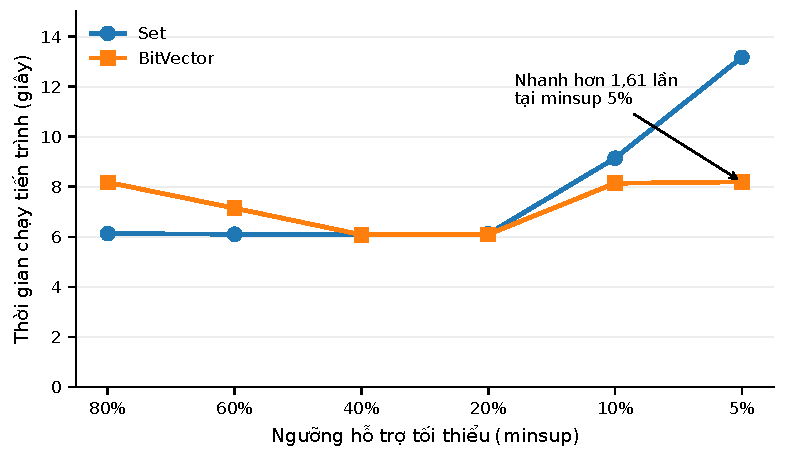
\includegraphics[width=\columnwidth]{figures/eclat/fig2_runtime_comparison.pdf}
    \caption{Thời gian thực thi của Set và BitVector theo ngưỡng hỗ trợ tối thiểu.}
    \label{fig:eclat_runtime}
\end{figure}

Bộ nhớ vật lý cực đại (peak RSS) của Set tăng từ 436,14 MiB ở 80\% lên 540,73 MiB ở 5\%. Số đo của BitVector dao động từ 432,62 đến 447,99 MiB qua sáu ngưỡng (Hình~\ref{fig:eclat_memory}).

\begin{figure}[!t]
    \centering
    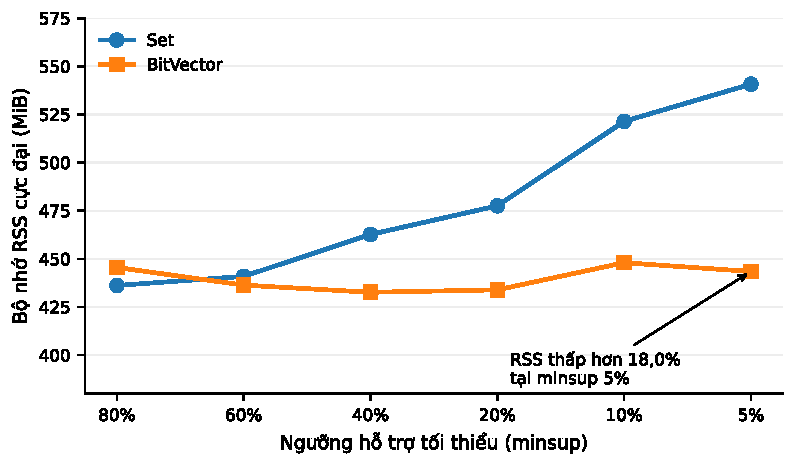
\includegraphics[width=\columnwidth]{figures/eclat/fig3_memory_comparison.pdf}
    \caption{Bộ nhớ vật lý cực đại của Set và BitVector theo ngưỡng hỗ trợ tối thiểu.}
    \label{fig:eclat_memory}
\end{figure}

Ở mỗi ngưỡng, nhóm chạy Set trước rồi chạy BitVector, mỗi bản một lượt với Julia 1.13.3, một luồng và giới hạn 3.072 MiB cho mỗi tiến trình. Thời gian đo bao gồm chuẩn bị đầu vào, khai thác và ghi kết quả. Phụ lục~\ref{app:fashion_eclat} trình bày kết quả đối chiếu và phạm vi phép đo.

\subsection{Phân tích và diễn giải mẫu trực quan}
\label{subsec:visual_pattern_interpretation}

Bảng~\ref{tab:visual_pattern_examples} trình bày bốn mẫu chọn từ kết quả Set sau khi gộp các ngưỡng và loại trùng. Nhóm chia danh sách thành chín nhóm theo ba khoảng độ dài (1, 2 và từ 3 mục trở lên) và ba mức hỗ trợ. Quy tắc ưu tiên lấy mẫu ở cả ba khoảng độ dài và giới hạn độ tương đồng Jaccard giữa hai mẫu ở mức 0,80. Phụ lục~\ref{app:fashion_patterns} minh họa thêm ba mẫu.

Để diễn giải mẫu, nhóm đặt mỗi tâm cụm dưới dạng lưới $4 \times 4$ cạnh những vùng ảnh thật được gán vào tâm đó. Trên ảnh gốc, các khung màu đánh dấu vị trí của những vùng này. Ảnh hỗ trợ chứa đầy đủ các từ thị giác trong mẫu, còn ảnh đối chứng thiếu ít nhất một từ.

Sau khi chốt tập mục cần minh họa, nhóm mới dùng nhãn lớp để chọn ảnh. Bộ ví dụ ưu tiên một ảnh thuộc lớp có tỷ lệ chứa mẫu cao nhất, rồi lấy thêm ảnh từ các lớp còn lại, với giá trị khởi tạo ngẫu nhiên 42 và tối đa sáu ảnh chứa mẫu. Bộ ảnh minh họa giúp xem vị trí và hình dạng các vùng được gán mã.

Nhóm dùng hệ số làm giàu (\textit{enrichment}) để so sánh tỷ lệ ảnh chứa tập mục $X$ trong lớp $c$ với tỷ lệ trên toàn bộ dữ liệu.
\begin{equation}
    E(X,c)=\frac{P(X\mid c)}{P(X)}
          =\frac{P(c\mid X)}{P(c)}.
    \label{eq:fim_F_class_enrichment}
\end{equation}
Trong công thức này, $P(X)$ là tỷ lệ ảnh chứa $X$ trên toàn bộ dữ liệu, $P(X\mid c)$ là tỷ lệ tương ứng trong lớp $c$, còn $P(c\mid X)$ là tỷ lệ ảnh thuộc lớp $c$ trong số những ảnh chứa $X$. Mỗi lớp có 7.000 ảnh nên $P(c)=10\%$. Hệ số $E$ lớn hơn 1 cho biết tập mục phổ biến hơn trong lớp đó so với toàn bộ dữ liệu. Bảng~\ref{tab:visual_pattern_examples} ghi lớp có hệ số cao nhất của từng mẫu.

\begin{table}[!t]
    \centering
    \caption{Độ hỗ trợ và lớp nổi bật của bốn mẫu đại diện}
    \label{tab:visual_pattern_examples}
    \footnotesize
    \setlength{\tabcolsep}{3pt}
    \begin{tabular}{l r l r}
        \hline
        \textbf{Tập mục} & \textbf{Độ hỗ trợ} &
        \textbf{Lớp nổi bật} & \textbf{Hệ số $E$} \\
        \hline
        $\{26\}$      & 69,89\% & Sandal     & $1{,}27\times$ \\
        $\{6\}$       & 61,80\% & Ankle boot & $1{,}31\times$ \\
        $\{1,24\}$    &  9,76\% & Sandal     & $2{,}27\times$ \\
        $\{4,12,24\}$ &  6,91\% & Ankle boot & $2{,}67\times$ \\
        \hline
    \end{tabular}
\end{table}

Hai tập đơn mục $\{26\}$ và $\{6\}$ lần lượt xuất hiện trong 48.922 ảnh (69,89\%) và 43.263 ảnh (61,80\%). Tâm cụm và các vùng ảnh minh họa gợi ý rằng cả hai mã biểu diễn những thay đổi sáng tối cục bộ có thể gặp ở nhiều lớp. Dù phổ biến trên toàn bộ dữ liệu, chúng xuất hiện ít hơn trong lớp Trouser, lần lượt ở 30,23\% và 9,97\% số ảnh của lớp.

Tập hai mục $\{1,24\}$ xuất hiện trong 6.829 ảnh (9,76\%) và có mặt ở cả 10 lớp. Trong lớp Sandal, tỷ lệ này đạt 22,19\%, gấp 2,27 lần mức chung.

Ở mẫu $\{4,12,24\}$, các tâm cụm gợi ý ba kiểu chuyển tiếp sáng tối, lần lượt gần mép trên, mép phải và mép dưới của vùng ảnh (Hình~\ref{fig:visual_pattern_4_12_24}). Mẫu xuất hiện trong 4.838 ảnh (6,91\%). Riêng lớp Ankle boot có 1.291 trong 7.000 ảnh chứa mẫu (18,44\%), gấp 2,67 lần tỷ lệ chung.

\begin{figure*}[!t]
    \centering
    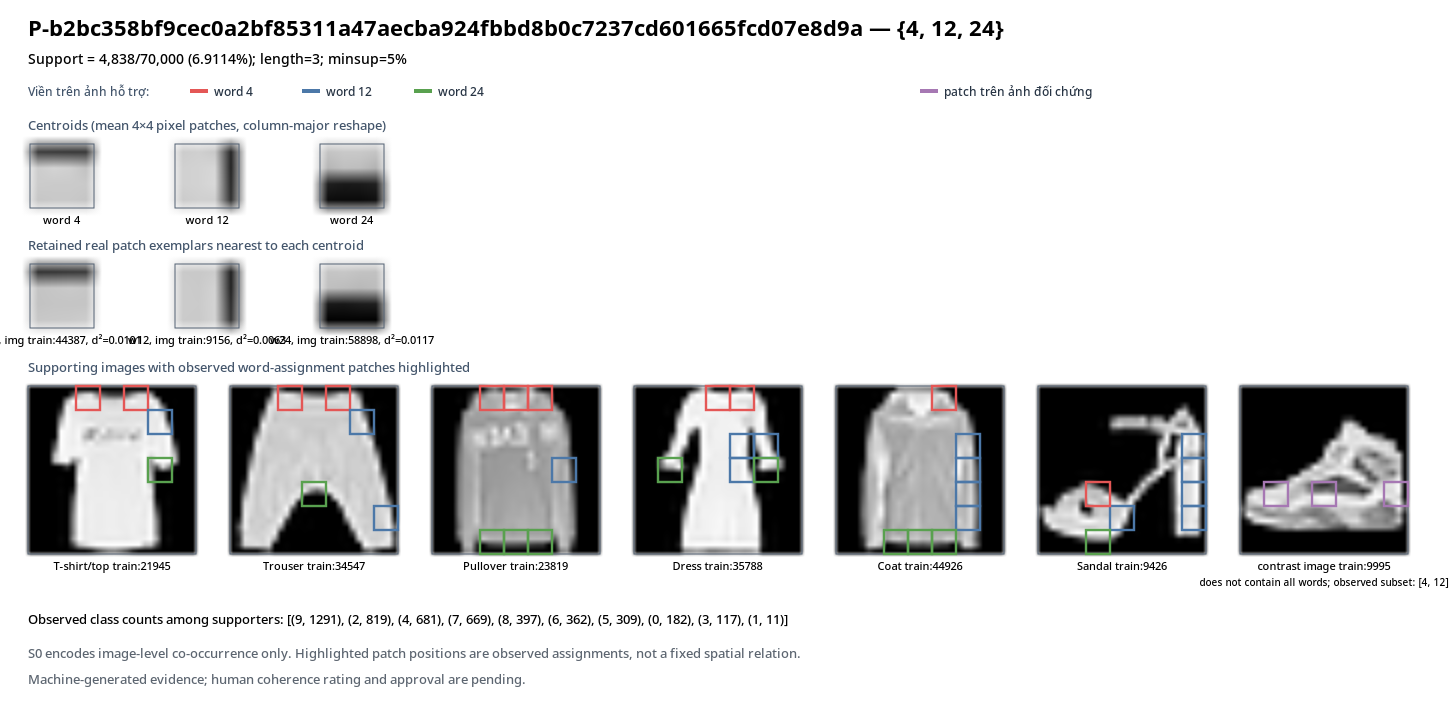
\includegraphics[width=0.98\textwidth]{figures/pattern_4_12_24.png}
    \caption{Tâm cụm, vùng ảnh thật, ảnh hỗ trợ và ảnh đối chứng của mẫu $\{4,12,24\}$. Khung màu đánh dấu vị trí các vùng được gán từ thị giác trong từng ảnh.}
    \label{fig:visual_pattern_4_12_24}
\end{figure*}

Hình~\ref{fig:visual_pattern_4_12_24} đặt cạnh nhau một ảnh Ankle boot chứa cả ba mã và một ảnh cùng lớp thiếu mã 24. Các vùng được đánh dấu nằm ở những vị trí khác nhau giữa các ảnh minh họa. Kết quả BoVW nhị phân cho biết ba mã có cùng xuất hiện trong ảnh hay không. Việc khảo sát bố cục cần dựa vào tọa độ của các vùng được gán mã.

\subsection{Phân tích theo lớp và thảo luận}
\label{subsec:fim_class_applications}

Sau khi xem xét bốn mẫu minh họa, nhóm mở rộng phân tích theo lớp sang toàn bộ 7.228 tập mục tìm được ở ngưỡng 5\%. Mỗi lớp có 7.000 ảnh và tổng số ảnh chứa từng tập mục qua mười lớp khớp với độ hỗ trợ do Eclat trả về.

Với mỗi tập mục $X$, nhóm tính hệ số làm giàu theo công thức~\eqref{eq:fim_F_class_enrichment} cho cả mười lớp và lấy giá trị cao nhất $E_{\max}(X)=\max_c E(X,c)$. Chẳng hạn, $E_{\max}(X)\geq 2$ nghĩa là có ít nhất một lớp mà tỷ lệ ảnh chứa $X$ cao gấp đôi mức chung trở lên.

\begin{table}[!t]
    \centering
    \caption{Hệ số làm giàu theo ngưỡng hỗ trợ tối thiểu}
    \label{tab:fim_F_class_summary}
    \footnotesize
    \setlength{\tabcolsep}{3.2pt}
    \begin{tabular}{c r r r}
        \toprule
        \textbf{Ngưỡng} & \textbf{Số tập mục} &
        \textbf{Trung vị $E_{\max}$} & \textbf{Số tập $E_{\max}\geq2$} \\
        \midrule
        80\% & 0     & --   & 0 \\
        60\% & 2     & 1,29 & 0 \\
        40\% & 15    & 1,46 & 0 \\
        20\% & 174   & 1,71 & 31 \\
        10\% & 1.275 & 1,91 & 506 \\
         5\% & 7.228 & 2,11 & 4.349 \\
        \bottomrule
    \end{tabular}
\end{table}

Bảng~\ref{tab:fim_F_class_summary} và Hình~\ref{fig:fim_F5_enrichment} cho thấy trung vị $E_{\max}$ là 1,71 ở ngưỡng 20\% và 2,11 ở ngưỡng 5\%. Tỷ lệ tập mục đạt $E_{\max}\geq 2$ lần lượt là 17,82\% (31 trên 174) và 60,17\% (4.349 trên 7.228). Các tập mục đã có ở ngưỡng 20\% giữ nguyên hệ số làm giàu. Chênh lệch phản ánh các mẫu ít phổ biến hơn được bổ sung khi hạ ngưỡng.

\begin{figure}[!t]
    \centering
    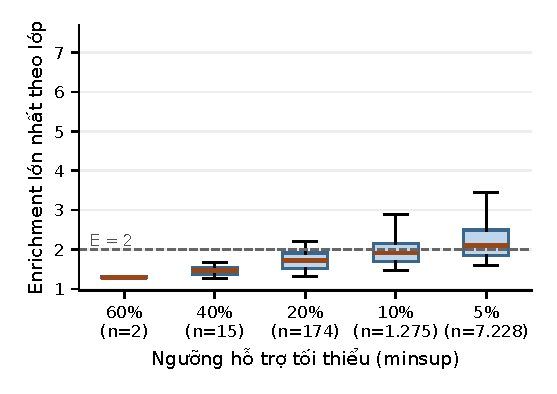
\includegraphics[width=\columnwidth]{figures/hinh_F5_enrichment_theo_minsup.pdf}
    \caption{Phân bố $E_{\max}$ ở năm ngưỡng có tập mục phổ biến. Hộp thể hiện khoảng tứ phân vị. Đường đứt đánh dấu $E_{\max}=2$.}
    \label{fig:fim_F5_enrichment}
\end{figure}

Ở ngưỡng 5\%, có 1.830 tập mục đạt $E(X,c)\geq 2$ với Ankle boot, 831 tập với Coat và 603 tập với Sandal. Bag và Shirt lần lượt có 115 và 145 tập (Hình~\ref{fig:fim_F6_class_counts}). Cùng một tập mục có thể được tính cho nhiều lớp, và nhiều tập có thể chia sẻ phần lớn mã từ thị giác. Các con số này mô tả mức độ phổ biến theo lớp. Khả năng phân loại cần được đánh giá riêng.

\begin{figure}[!t]
    \centering
    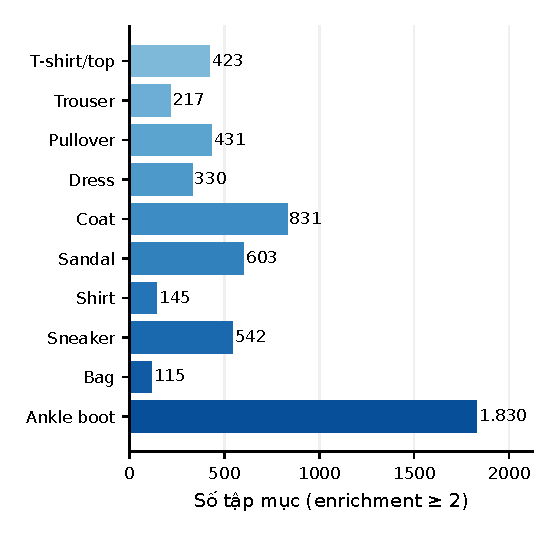
\includegraphics[width=\columnwidth]{figures/hinh_F6_so_tap_enrichment_theo_lop.pdf}
    \caption{Số tập mục đạt $E(X,c)\geq 2$ trong từng lớp, tính trên 7.228 tập mục ở ngưỡng hỗ trợ 5\%.}
    \label{fig:fim_F6_class_counts}
\end{figure}

Để minh họa từng lớp, nhóm bắt đầu từ 7.228 tập mục ở ngưỡng 5\%. Nhóm chỉ xét những tập có ít nhất hai mục và xuất hiện trong ít nhất 10\% ảnh của lớp đó, rồi chọn tập có $E(X,c)$ cao nhất. Hình~\ref{fig:fim_F7_class_heatmap} cho thấy tỷ lệ ảnh chứa mười mẫu được chọn trong từng lớp.

\twocolumn[{%
\begin{minipage}{\textwidth}
    \centering
    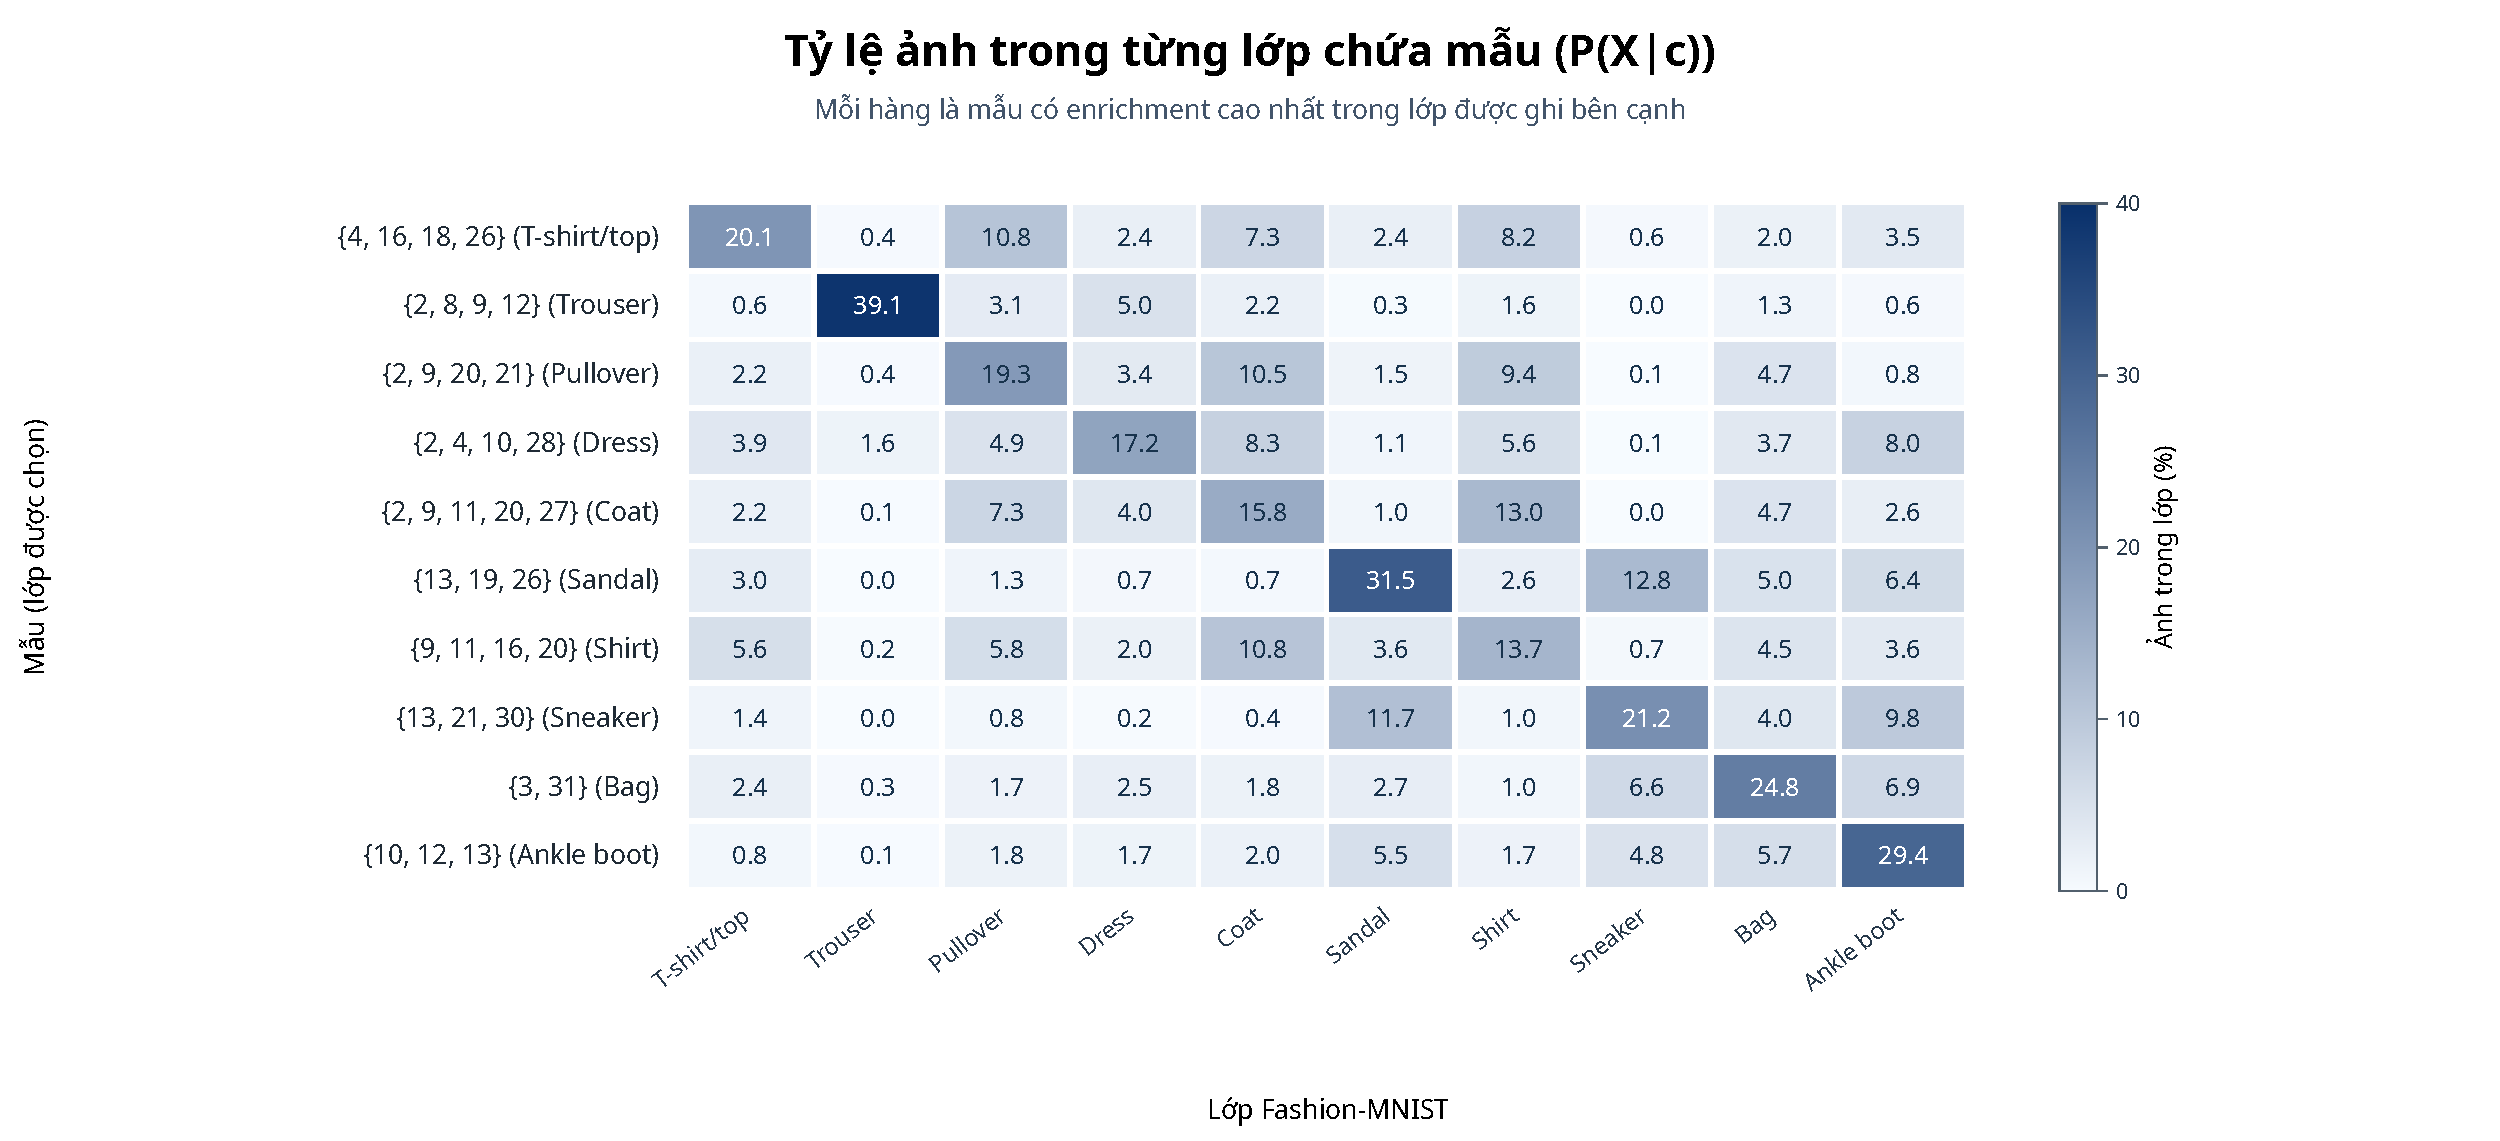
\includegraphics[width=\textwidth]{figures/hinh_F7_heatmap_mau_theo_lop.pdf}
    \captionof{figure}{Tỷ lệ ảnh của từng lớp chứa mỗi mẫu minh họa. Mỗi hàng là tập có hệ số làm giàu cao nhất với lớp ghi trong ngoặc, trong số các tập có ít nhất hai mục và xuất hiện trong ít nhất 10\% ảnh của lớp đó.}
    \label{fig:fim_F7_class_heatmap}
\end{minipage}\par\bigskip
}]

Hai hàng trong Hình~\ref{fig:fim_F7_class_heatmap} cho thấy mức độ tập trung khác nhau. Mẫu $\{2,8,9,12\}$ xuất hiện ở 39,1\% ảnh Trouser, còn tỷ lệ cao nhất ở các lớp khác là 5,0\% (Dress). Mẫu $\{2,9,11,20,27\}$ xuất hiện ở 15,8\% ảnh Coat và cũng có mặt ở 13,0\% ảnh Shirt.

\textit{Hướng nghiên cứu tiếp theo.} Có thể dùng sự hiện diện của từng tập mục làm đặc trưng nhị phân cho bài toán phân loại ảnh. Với $m$ tập mục được chọn, đặc trưng thứ $j$ của ảnh $I_i$ cho biết giao dịch $T_i$ có chứa tập mục $P_j$ hay không.
\begin{equation}
    \phi_j(I_i)=\mathbf{1}\!\left[P_j\subseteq T_i\right],
    \qquad j=1,\ldots,m.
    \label{eq:fim_F_class_activation}
\end{equation}
Một thí nghiệm phân loại độc lập có thể dùng hồi quy logistic đa lớp để so sánh BoVW, đặc trưng tập mục và tổ hợp của cả hai bằng độ chính xác và Macro-F1. Cần tách tập huấn luyện và kiểm thử ngay từ đầu. Việc ước lượng ngưỡng lọc, học từ điển, khai thác tập mục và chọn đặc trưng chỉ dùng tập huấn luyện. Cấu hình đã chốt được áp dụng lên tập kiểm thử để đánh giá dự đoán.

\section{Kết luận}

Hai bản cài đặt Eclat cho cùng kết quả ở cả sáu ngưỡng hỗ trợ. Trong 7.228 tập mục ở ngưỡng 5\%, một số tổ hợp từ thị giác xuất hiện nhiều hơn hẳn ở một lớp. Chẳng hạn, mẫu $\{2,8,9,12\}$ có mặt trong 39,1\% ảnh Trouser, so với 5,4\% trên toàn bộ tập ảnh.

Các kết quả mô tả sự đồng xuất hiện của từ thị giác trong 70.000 ảnh dùng để học từ điển và khai thác mẫu. BoVW nhị phân bỏ qua số lần lặp và vị trí của các từ trong ảnh. Để đánh giá giá trị phân loại của các mẫu, cần một tập kiểm thử độc lập.


% \section*{Acknowledgment}

% The preferred spelling of the word ``acknowledgment'' in America is without
% an ``e'' after the ``g''. Avoid the stilted expression ``one of us (R. B.
% G.) thanks $\ldots$''. Instead, try ``R. B. G. thanks$\ldots$''. Put sponsor
% acknowledgments in the unnumbered footnote on the first page.
\begin{thebibliography}{99}
\bibitem{Sivic03}
J. Sivic and A. Zisserman,
``Video Google: A Text Retrieval Approach to Object Matching in Videos,''
in \textit{Proc. IEEE International Conference on Computer Vision (ICCV)},
vol. 2, pp. 1470--1477, 2003.

\bibitem{Hartigan1979}
J. A. Hartigan and M. A. Wong,
``Algorithm AS 136: A K-Means Clustering Algorithm,''
\textit{Journal of the Royal Statistical Society,
Series C (Applied Statistics)},
vol. 28, no. 1, pp. 100--108, 1979,
doi: 10.2307/2346830.


\bibitem{Xiao2017}
H. Xiao, K. Rasul, and R. Vollgraf,
``Fashion-MNIST: A Novel Image Dataset for Benchmarking
Machine Learning Algorithms,''
\textit{arXiv preprint arXiv:1708.07747}, 2017,
doi: 10.48550/arXiv.1708.07747.


\end{thebibliography}

\clearpage
\appendices

\section{Khảo sát cấu hình và đặc điểm giao dịch}
\label{app:fashion_configuration}

\textit{Kích thước vùng ảnh.}
Lưới không chồng lấn trên ảnh $28\times28$ tạo 196, 49 hoặc 16 vùng khi cạnh vùng lần lượt là 2, 4 hoặc 7 pixel. Vùng nhỏ cho phép lọc nền chi tiết hơn nhưng làm tăng số vectơ cần xử lý. Vùng lớn chứa nhiều điểm ảnh lân cận hơn và có thể trộn nền với các đường biên của vật thể. Trong phép đối chiếu $4\times4$ với $7\times7$, ở mức loại khoảng 39,3\% số vùng, tỷ lệ gradient bị mất lần lượt là 5,92\% và 14,00\%. Lưới cố định cũng khiến mẫu điểm ảnh phụ thuộc vào vị trí của đường biên so với lưới.

\textit{Lọc nền.}
Bảng~\ref{tab:fashion_filter_appendix} so sánh các cấu hình trong khảo sát ảnh. Tỷ lệ mất gradient được tính bằng tổng độ lớn gradient trong các vùng bị loại chia cho tổng độ lớn gradient trên ảnh gốc. Với ngưỡng 29, mỗi ảnh còn trung bình 30,62 vùng và mọi ảnh đều còn ít nhất một vùng.

\begin{center}
    \captionof{table}{Ảnh hưởng của ngưỡng lọc trên lưới $4\times4$}
    \label{tab:fashion_filter_appendix}
    \footnotesize
    \begin{tabular}{@{}lrrr@{}}
        \toprule
        Cấu hình & Vùng loại & Mất gradient & Mất hết vùng \\
        \midrule
        Giữ mọi vùng      & 0,00\%  & 0,00\% & 0 \\
        Ngưỡng 29 (Q10+) & 37,50\% & 4,41\% & 0 \\
        Ngưỡng 97 (Otsu) & 43,30\% & 8,90\% & 0 \\
        \bottomrule
    \end{tabular}
\end{center}

\textit{Đặc trưng và số cụm.}
Vectơ gồm 16 mức xám theo thứ tự cột, vì vậy bình phương khoảng cách Euclid cộng chênh lệch bình phương tại các vị trí tương ứng. Biểu diễn này giữ bố cục điểm ảnh trong vùng nhỏ và nhạy với thay đổi độ sáng, dịch chuyển hoặc xoay. Bảng~\ref{tab:fashion_k_appendix} ghi kết quả khảo sát ở cùng giá trị khởi tạo ngẫu nhiên 123. Khi số cụm tăng, các lượt khảo sát cho độ méo thấp hơn và giao dịch dài hơn.

\begin{center}
    \captionof{table}{Đánh đổi giữa độ méo và độ dài giao dịch}
    \label{tab:fashion_k_appendix}
    \footnotesize
    \begin{tabular}{@{}rrrr@{}}
        \toprule
        $K$ & Độ méo & Số mã TB & Hội tụ \\
        \midrule
        16  & 0,441 &  9,00 & Có \\
        32  & 0,347 & 12,27 & Có \\
        64  & 0,271 & 15,11 & Có \\
        128 & 0,219 & 17,99 & Có \\
        256 & 0,177 & 20,29 & Chưa \\
        \bottomrule
    \end{tabular}
\end{center}

\textit{Giao dịch dùng trong báo cáo.}
Sau khi bỏ các mã lặp trong từng ảnh, 70.000 giao dịch có tổng cộng 859.100 lượt xuất hiện của 32 mã phân biệt. Độ dài giao dịch từ 2 đến 26, với trung vị 12 và độ lệch chuẩn 3,06 mã. Mật độ, tính bằng $859\,100/(70\,000\times32)$, là 38,35\%.
Thống kê trên được tính trực tiếp từ bộ giao dịch dùng trong báo cáo.
Xem \href{https://github.com/NguyenVoTanDuy2006/DataMining-FIM-Project/blob/e8390ba36d55e79c3ea8258d4d56de6385a8b733/docs/UD2/TC_plan.md}{khảo sát tiền xử lý ảnh} và \href{https://github.com/NguyenVoTanDuy2006/DataMining-FIM-Project/blob/e8390ba36d55e79c3ea8258d4d56de6385a8b733/notebook/UD2/experiments/EDA2_FashionMNIST_Transaction_Evaluation.ipynb}{khảo sát giao dịch}.

\newpage
\section{Đối chiếu Eclat và cách đọc số đo}
\label{app:fashion_eclat}

\textit{Độ hỗ trợ trên BoVW nhị phân.}
Gọi $D(w)$ là tập giao dịch chứa từ thị giác $w$ và $N$ là số giao dịch. Độ hỗ trợ của tập mục $X$ là
\[
    \operatorname{supp}(X)
    = \frac{\left|\bigcap_{w\in X} D(w)\right|}{N}.
\]
Ví dụ minh họa, với ba giao dịch $\{1,6\}$, $\{6,24\}$ và $\{1,6,24\}$, cặp $\{1,6\}$ xuất hiện ở giao dịch thứ nhất và thứ ba nên có độ hỗ trợ $2/3$. Histogram tần suất giữ được số lần lặp và cần thêm quy tắc mã hóa nếu dùng với Eclat. BoVW theo vùng giữ vị trí gần đúng bằng cách gắn mã với từng vùng. Cách này làm tăng số mục và có thể chia lượt xuất hiện của một mã giữa nhiều mục.

\textit{Đối chiếu kết quả.}
Nhóm chạy hai \href{https://github.com/NguyenVoTanDuy2006/DataMining-FIM-Project/tree/e8390ba36d55e79c3ea8258d4d56de6385a8b733/src/algorithm}{bản cài đặt Eclat} trên cùng một bộ giao dịch. Ở cả sáu ngưỡng, hai bản trả về cùng các tập mục và cùng số ảnh chứa từng tập. Cột \emph{Sai hỗ trợ} trong Bảng~\ref{tab:fashion_audit_appendix} ghi số tập mục có độ hỗ trợ tính lại khác với kết quả đã trả về.

\begin{center}
    \captionof{table}{Đối chiếu độ hỗ trợ và RSS theo ngưỡng}
    \label{tab:fashion_audit_appendix}
    \footnotesize
    \setlength{\tabcolsep}{3.5pt}
    \begin{tabular}{@{}rrrrr@{}}
        \toprule
        Ngưỡng & Số tập & Sai hỗ trợ & Set (MiB) & BitVector (MiB) \\
        \midrule
        80\% &     0 & 0 & 436,14 & 445,52 \\
        60\% &     2 & 0 & 440,89 & 436,34 \\
        40\% &    15 & 0 & 462,65 & 432,62 \\
        20\% &   174 & 0 & 477,53 & 433,88 \\
        10\% & 1.275 & 0 & 521,41 & 447,99 \\
         5\% & 7.228 & 0 & 540,73 & 443,43 \\
        \bottomrule
    \end{tabular}
\end{center}

\textit{Diễn giải thời gian và bộ nhớ.}
Khi thêm một mục, số giao dịch chứa tập mới chỉ có thể giữ nguyên hoặc giảm. Hạ ngưỡng giúp nhiều nhánh vượt qua bước cắt tỉa, nên Eclat có thể phải xét thêm các phép giao. Bản Set giao các tập số nguyên. Bản BitVector đếm trước các mục đơn để chỉ cấp phát vectơ bit cho những mục đạt ngưỡng, rồi dùng phép AND và đếm bit bật. Chi phí giao có thể góp phần vào chênh lệch quan sát được ở ngưỡng 5\%.

Mỗi cấu hình được đo một lượt trong một tiến trình riêng, chạy Julia 1.13.3 trên Linux với một luồng và giới hạn 3.072 MiB. Tổng thời gian bao gồm khởi tạo, nạp dữ liệu, khai thác và ghi kết quả. RSS đo lượng bộ nhớ vật lý cực đại của cả tiến trình. Để biết mức chênh lệch có ổn định hay không, cần đo lặp từng cấu hình. Xem \href{https://github.com/NguyenVoTanDuy2006/DataMining-FIM-Project/blob/e8390ba36d55e79c3ea8258d4d56de6385a8b733/notebook/UD2/release/03_frequent_itemset_mining.ipynb}{notebook thực nghiệm Eclat}.

\onecolumn
\section{Hình minh họa bổ sung cho các mẫu đại diện}
\label{app:fashion_patterns}

Ba hình dưới đây bổ sung cho Hình~\ref{fig:visual_pattern_4_12_24} trong thân bài. Mỗi hình đặt tâm cụm và vùng ảnh thật cạnh các ảnh chứa mẫu. Ảnh ngoài cùng bên phải thiếu ít nhất một mã của mẫu.

\begin{center}
    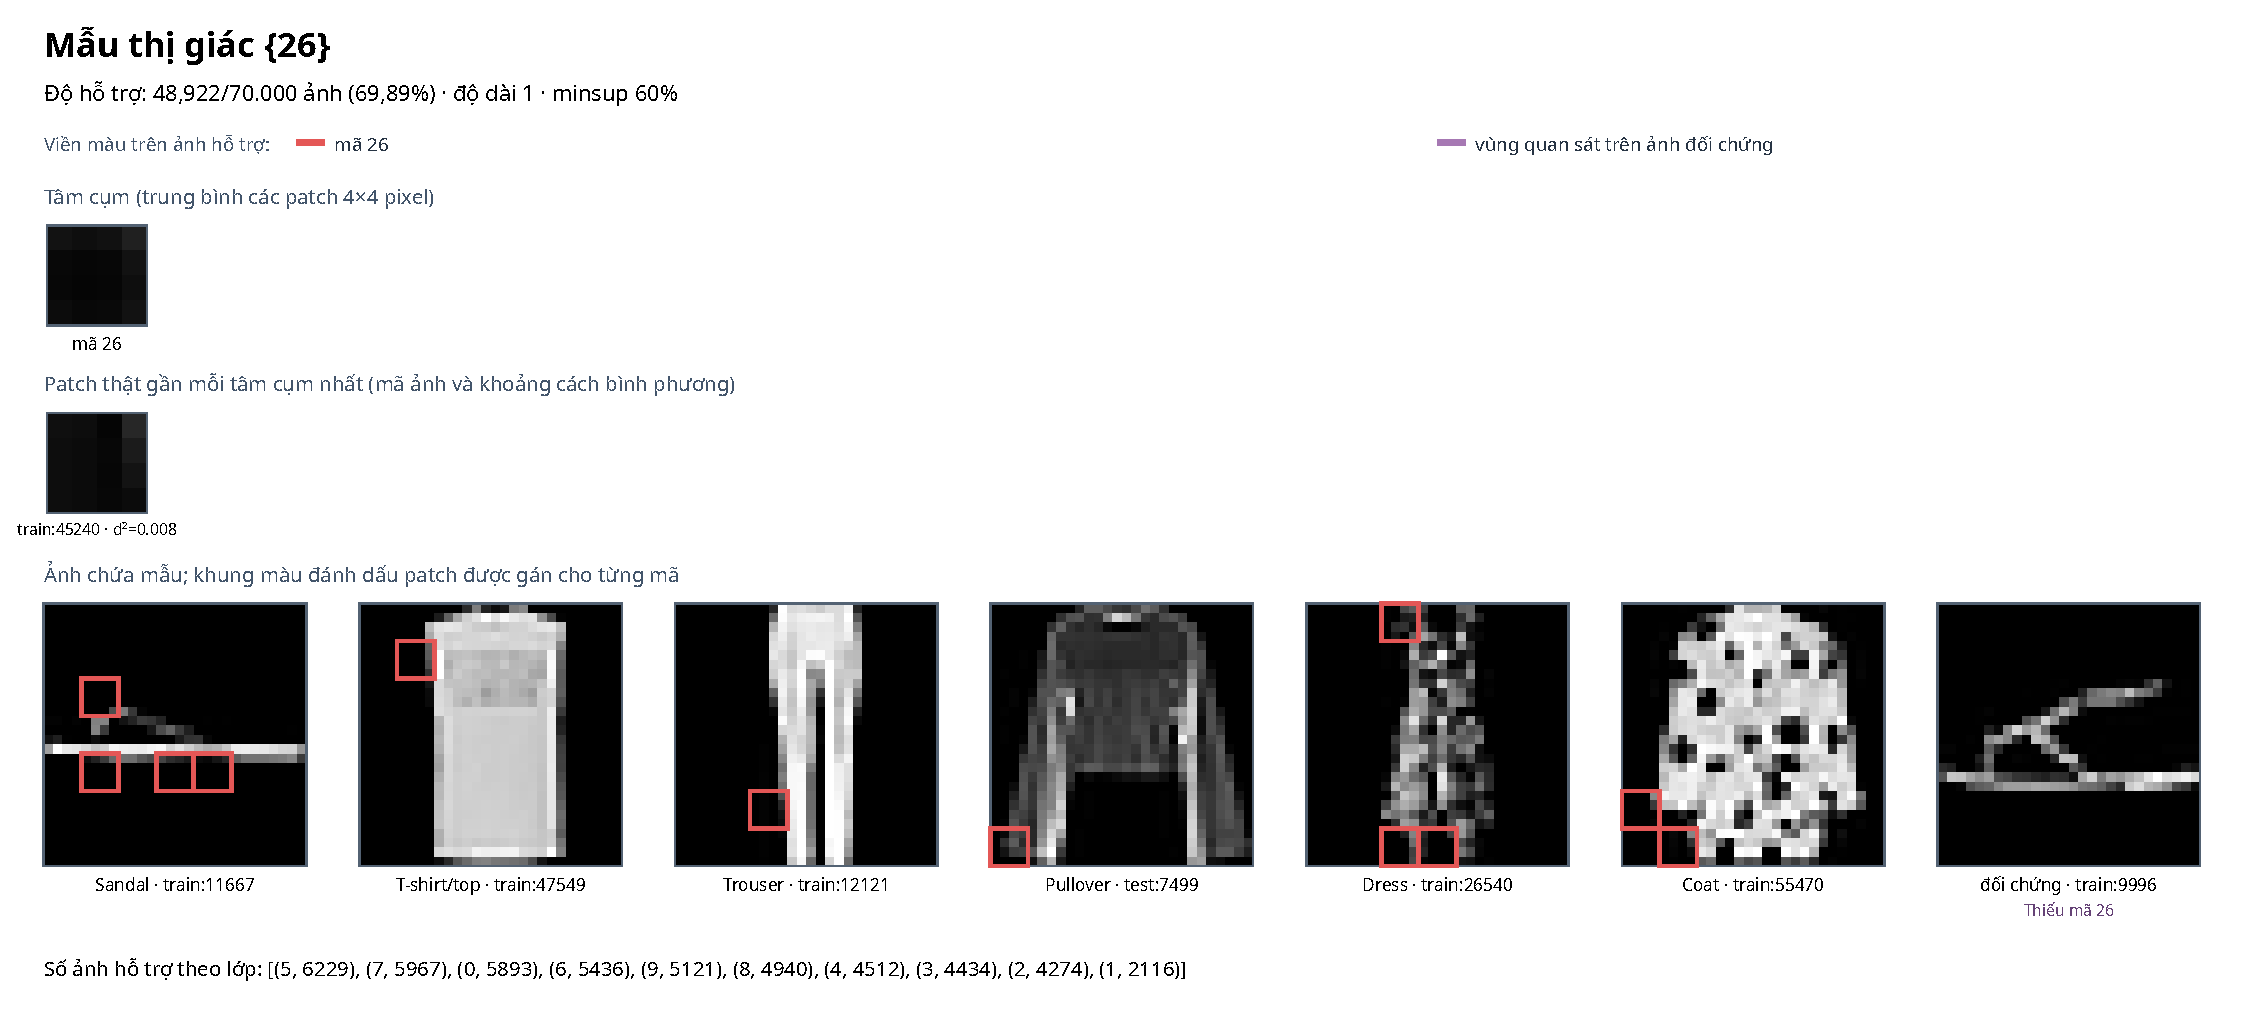
\includegraphics[width=0.97\textwidth,height=0.25\textheight,keepaspectratio]{figures/appendix/pattern_26.pdf}
    \captionof{figure}{Mẫu $\{26\}$. Tâm cụm chủ yếu có mức xám thấp. Các vùng gán mã 26 xuất hiện ở nhiều vị trí, chẳng hạn gần quai dép hoặc mép áo trong các ảnh minh họa.}
    \label{fig:fashion_appendix_26}
\end{center}

\begin{center}
    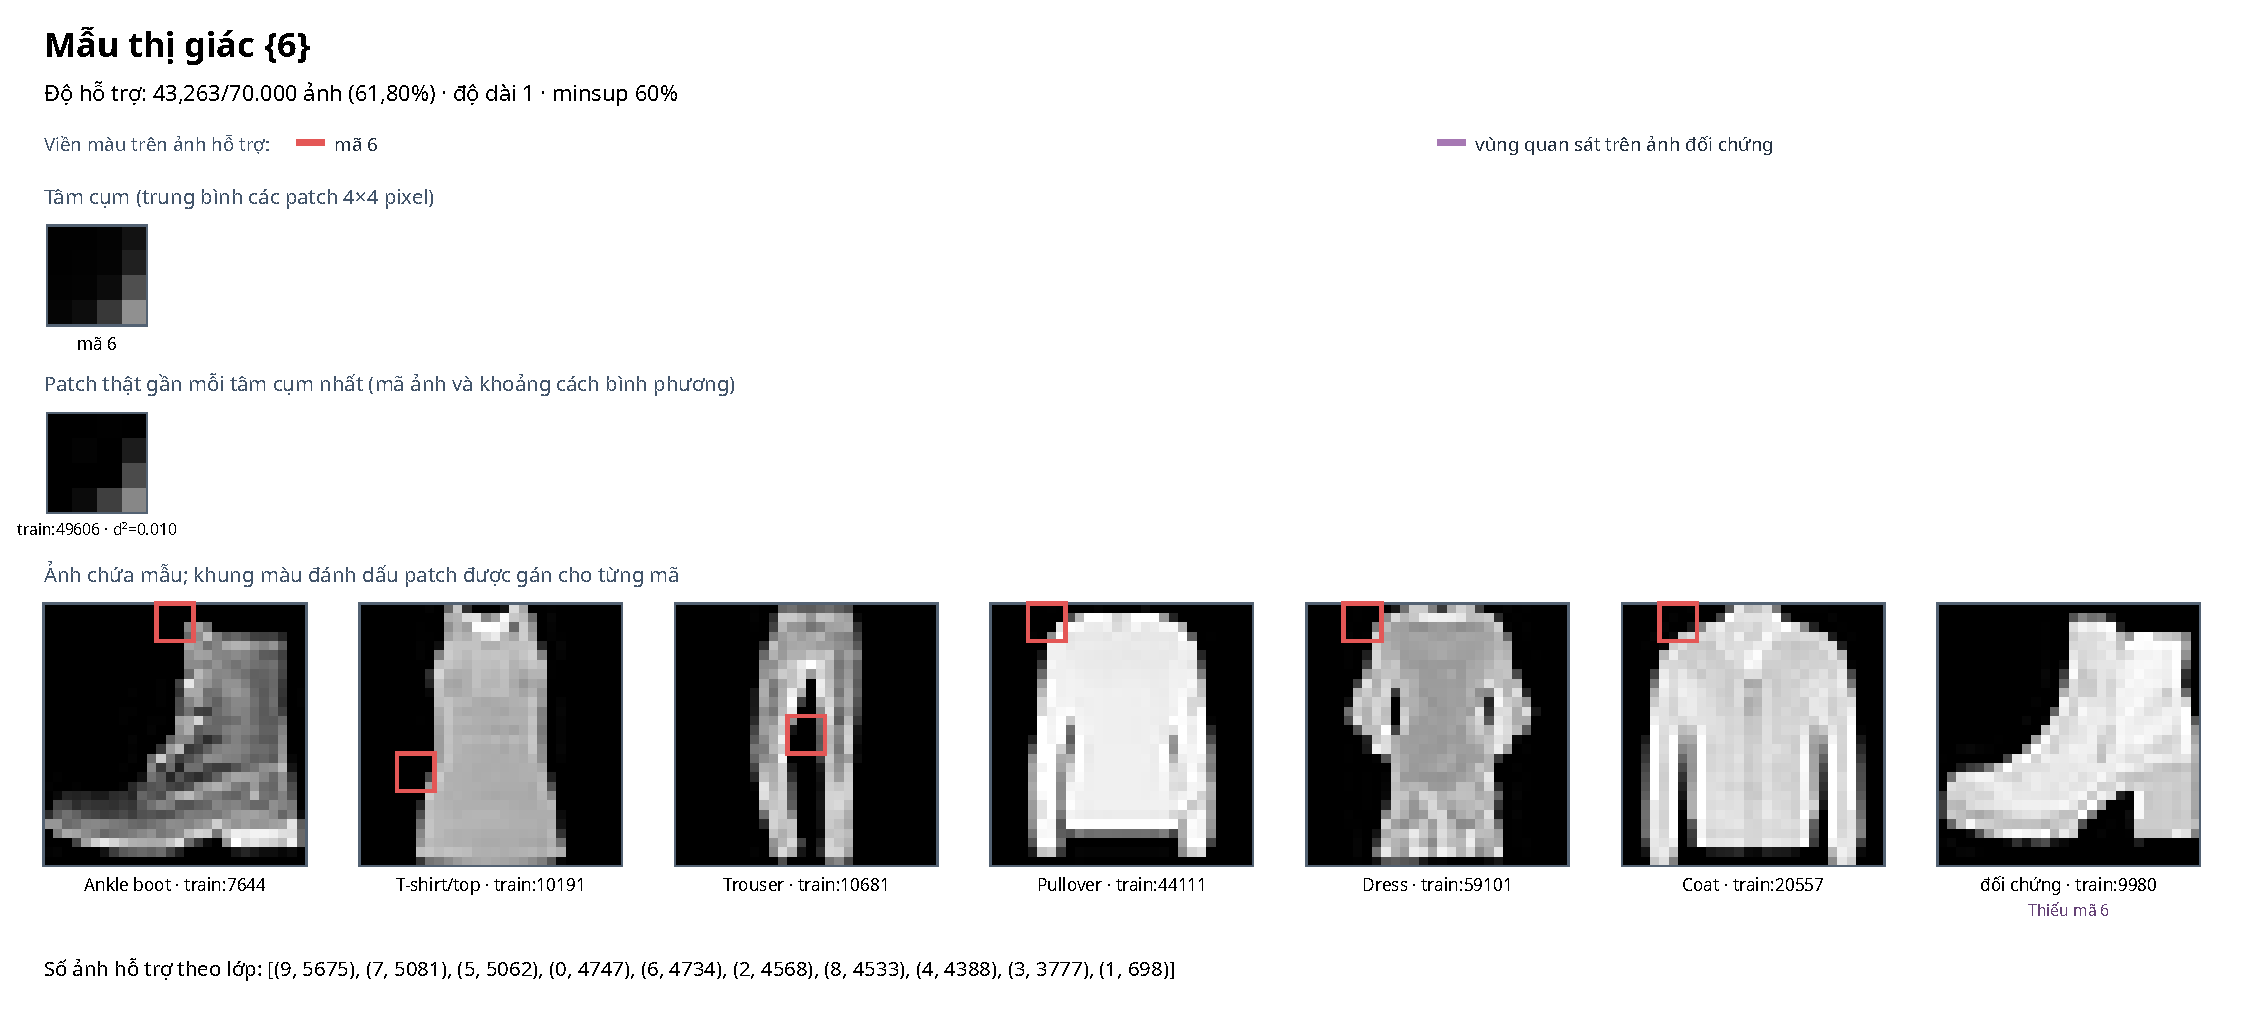
\includegraphics[width=0.97\textwidth,height=0.25\textheight,keepaspectratio]{figures/appendix/pattern_6.pdf}
    \captionof{figure}{Mẫu $\{6\}$. Tâm cụm chuyển từ vùng tối sang vùng sáng hơn ở một góc. Các vùng được đánh dấu cho thấy dạng chuyển mức xám này xuất hiện trên nhiều loại trang phục.}
    \label{fig:fashion_appendix_6}
\end{center}

\begin{center}
    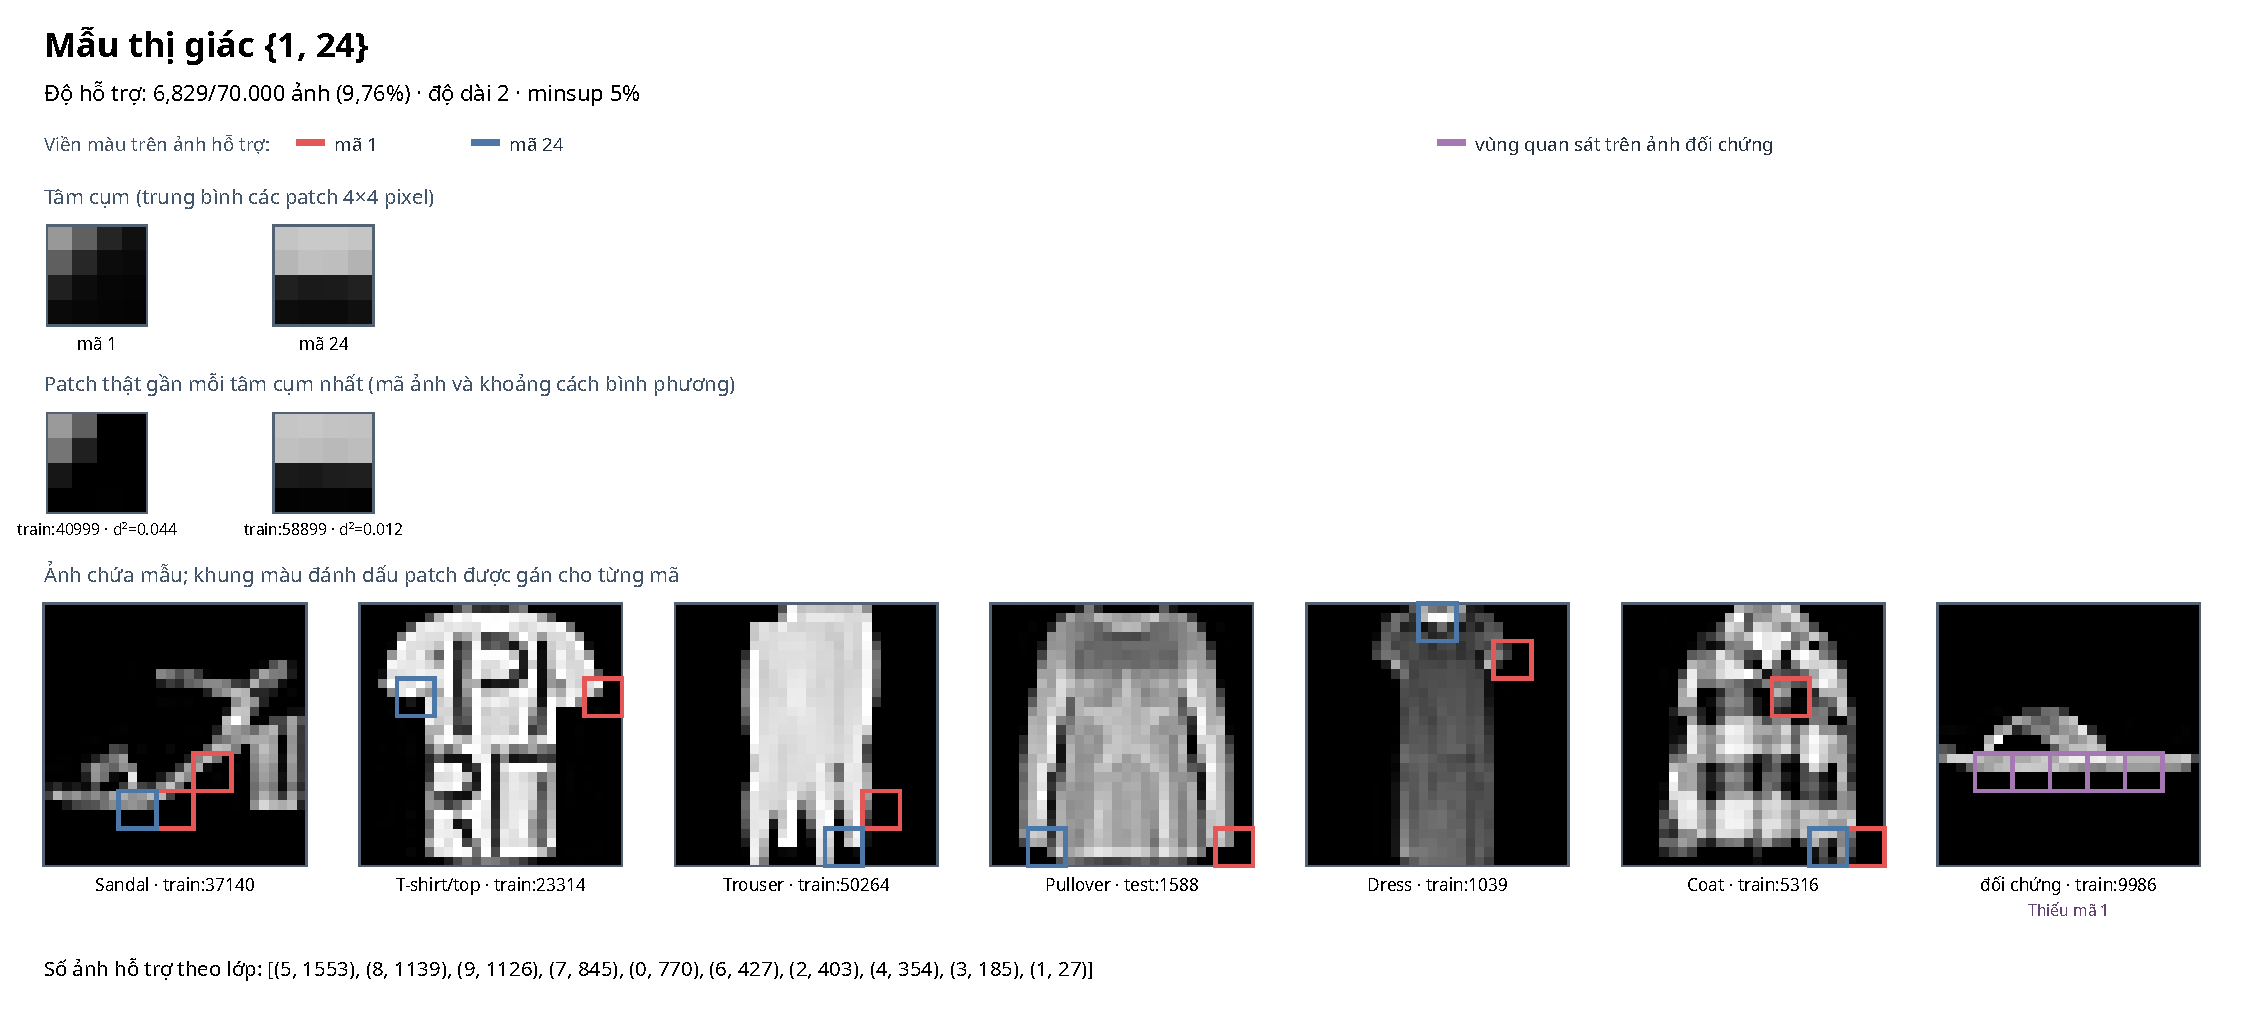
\includegraphics[width=0.97\textwidth,height=0.25\textheight,keepaspectratio]{figures/appendix/pattern_1_24.pdf}
    \captionof{figure}{Mẫu $\{1,24\}$. Mã 1 thể hiện chuyển sáng tối theo đường chéo, còn mã 24 có dải tối ở phần dưới. Các vùng mang hai mã có thể nằm ở những vị trí khác nhau trong cùng ảnh.}
    \label{fig:fashion_appendix_1_24}
\end{center}

\end{document}
